\documentclass[compress]{beamer}
\usepackage{graphicx}
\usepackage{graphics}
\usepackage{hyperref}
\usepackage{color}
\usepackage[english]{babel}
\usepackage{subfigure}
\usepackage{verbatim}
\usepackage{isomath,commath,amsmath,amssymb}


\newenvironment{wideitemize}{\itemize\addtolength{\itemsep}{10pt}}{\enditemize}

\mode<presentation>
{
\usetheme{UK}
\setbeamercovered{transparent = 28}
}

\def\vec#1{\mathchoice{\mbox{\boldmath$\displaystyle\bf#1$}}
{\mbox{\boldmath$\textstyle\bf#1$}}
{\mbox{\boldmath$\scriptstyle\bf#1$}}
{\mbox{\boldmath$\scriptscriptstyle\bf#1$}}}


\title{Edge Latents Guided Graph Attention Networks}
\subtitle{STA-695 Final Project}
\author{Jiaying Weng, Liyu Gong}\institute{Department of Statistics\\ University of Kentucky}
\date{}


\begin{document}

%%\begin{withoutheadline}
%\begin{frame}[plain]
%%\begin{frame}
%%\titlepage
%%\end{frame}
%%\end{withoutheadline}

{
\begin{withoutheadline}
	\begin{frame}
        \titlepage
    \end{frame} 
\end{withoutheadline}
} 

{
   \begin{frame}
       \frametitle{Outline}
       \tableofcontents
   \end{frame}
}

\AtBeginSection[]
{
   \begin{frame}
       \frametitle{Outline}
       \tableofcontents[currentsection]
   \end{frame}
}

\section{Introduction to graph and graph learning}

\begin{frame}
\frametitle{Graph}
\begin{itemize}
\item A graph is a structure amounting to a set of objects in which some pairs of the objects are in some sense ``related''.
\item Components
  \begin{itemize}
  \item Nodes (vertices, points)
  \item Edges (arcs, lines)
  \end{itemize}
\item Graph learning
  \begin{itemize}
  \item Node classification (regression)
  \item Edge classification (regression)
  \item Graph classification (regression)
  \item Node clustering
  \item \ldots
  \end{itemize}
\end{itemize}
\end{frame}

\begin{frame}
  \frametitle{Social network}
  \begin{center}
    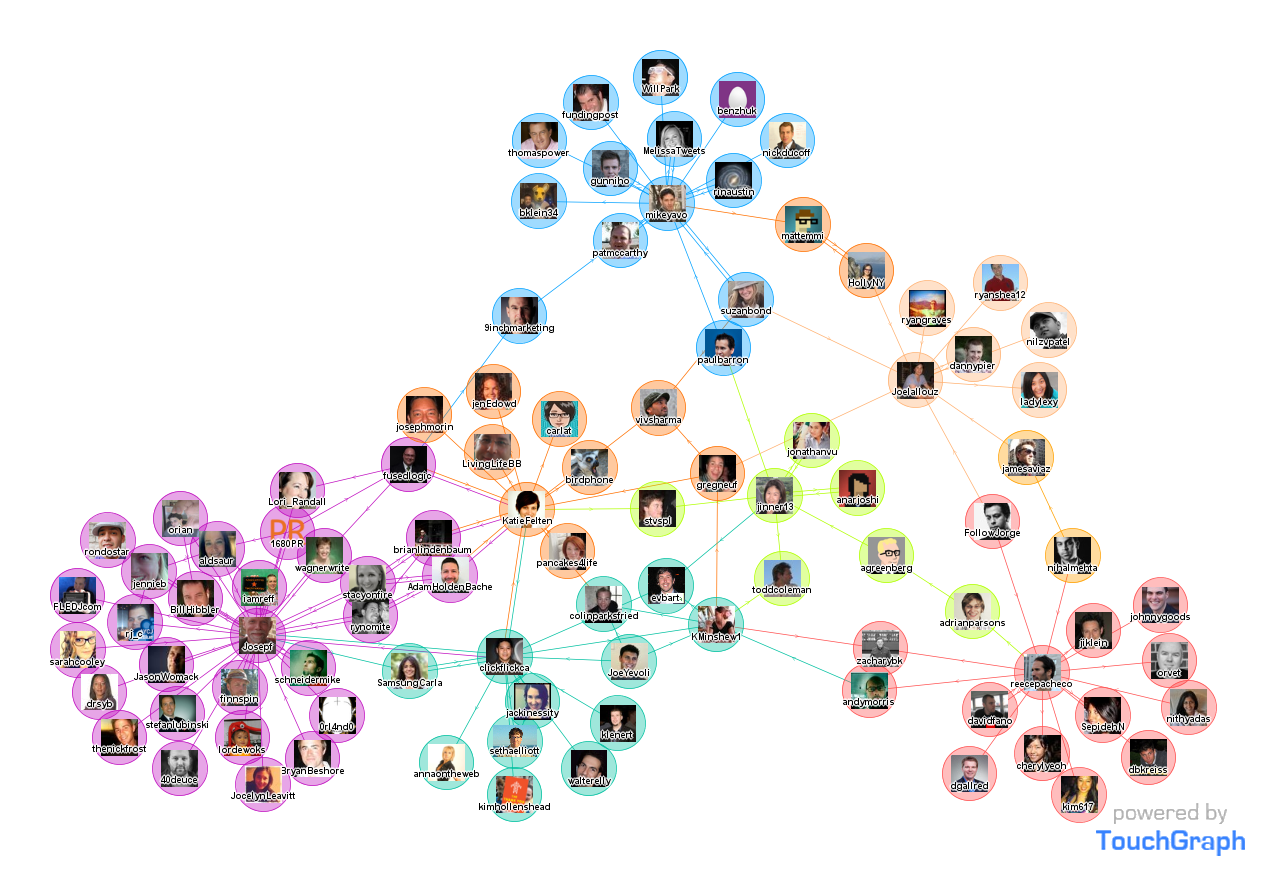
\includegraphics[scale=0.2]{social.png}
  \end{center}
\end{frame}

\begin{frame}
  \frametitle{Protein-protein interaction}
  \begin{center}
    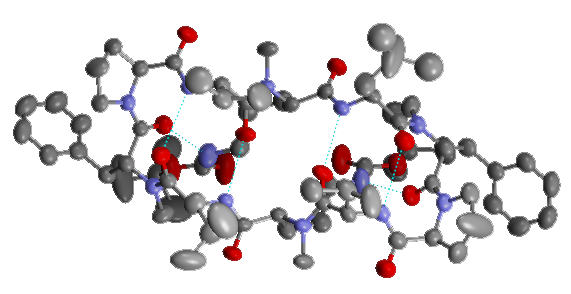
\includegraphics[scale=0.5]{ppi.png}
  \end{center}
\end{frame}

\begin{frame}
  \frametitle{Citation graph}
  \begin{center}
    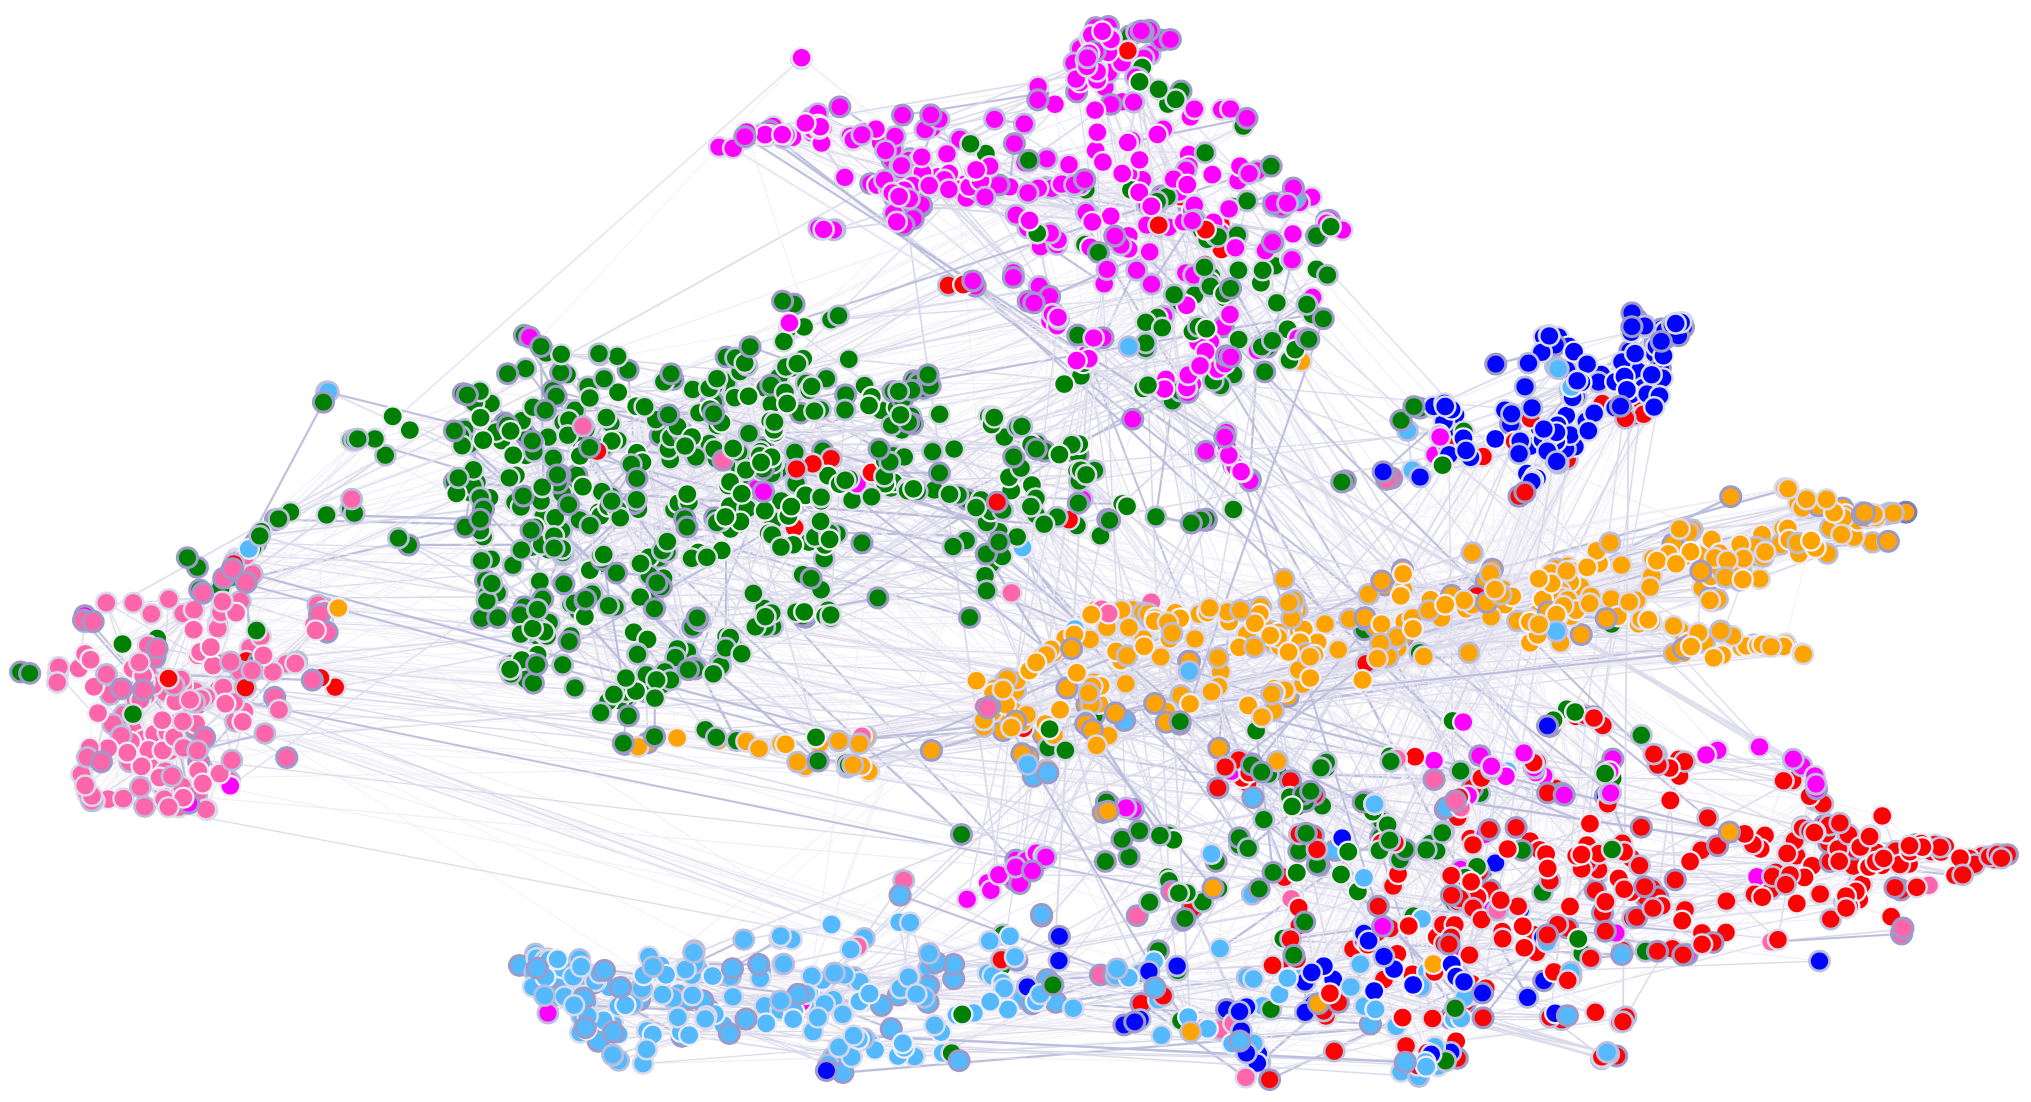
\includegraphics[scale=0.10]{citation.png}
  \end{center}
  \begin{itemize}
  \item Node: Paper
  \item Edge: Citation
  \end{itemize}
\end{frame}
\section{Introduction to attention mechanism}

\begin{frame}
\frametitle{Attention mechanism}
\begin{itemize}
\item Hot and new topic in deep learning
\item Successfully applied to machine translation problem
\item A learnable mechanism to aggregate features
\item Aggregate by weighted average
\item The weights for aggregating is a function of features
\item different content of features will have different weights (attention)
\end{itemize}
\end{frame}

\begin{frame}
  \frametitle{RNN based machine translation}
  \begin{itemize}
  \item Input sequence are encoded into a single vector by RNN
  \item Output sequence are generated from this vector by RNN
  \end{itemize}
  \begin{center}
    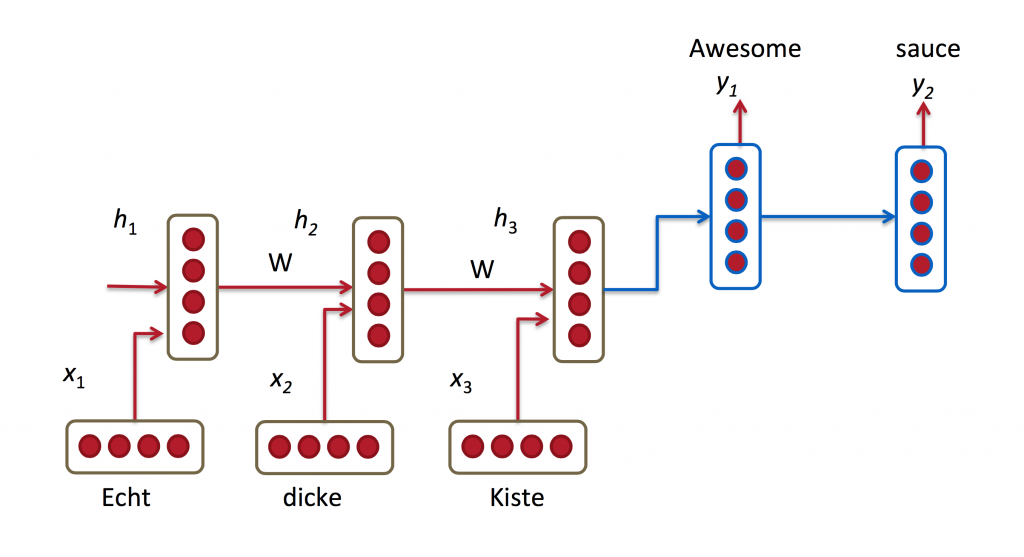
\includegraphics[scale=0.3]{translation.png}
  \end{center}
\end{frame}

\begin{frame}
  \frametitle{Why attention mechanism?}
  \begin{itemize}
  \item The RNN (LSTM) based method surprisingly works well!
  \item But, obviously, there is space for improvement
    \begin{alertblock}{Problem}
      The dependency between output sequence and input sequence is
      complex which could not be captured by the encoding RNN
    \end{alertblock}
    \begin{block}{Attention mechanism}
      \begin{itemize}
      \item Instead of using the last encoded vector, aggregate a
        feature vector from all the previous hidden states each time
        generating an output
      \item Aggregating could be a weighted average
      \item Weights are a trainable function of the contents
      \end{itemize}
    \end{block}
  \end{itemize}
\end{frame}

\begin{frame}
  \frametitle{Machine translation with attention mechanism}
  \begin{center}
    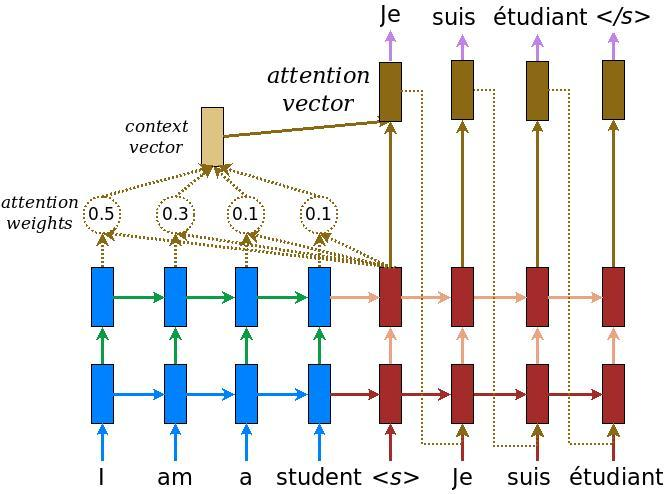
\includegraphics[scale=0.3]{translation_att.png}
  \end{center}
\end{frame}

\begin{frame}
  \frametitle{Interpreting attention weights}
  \begin{center}
    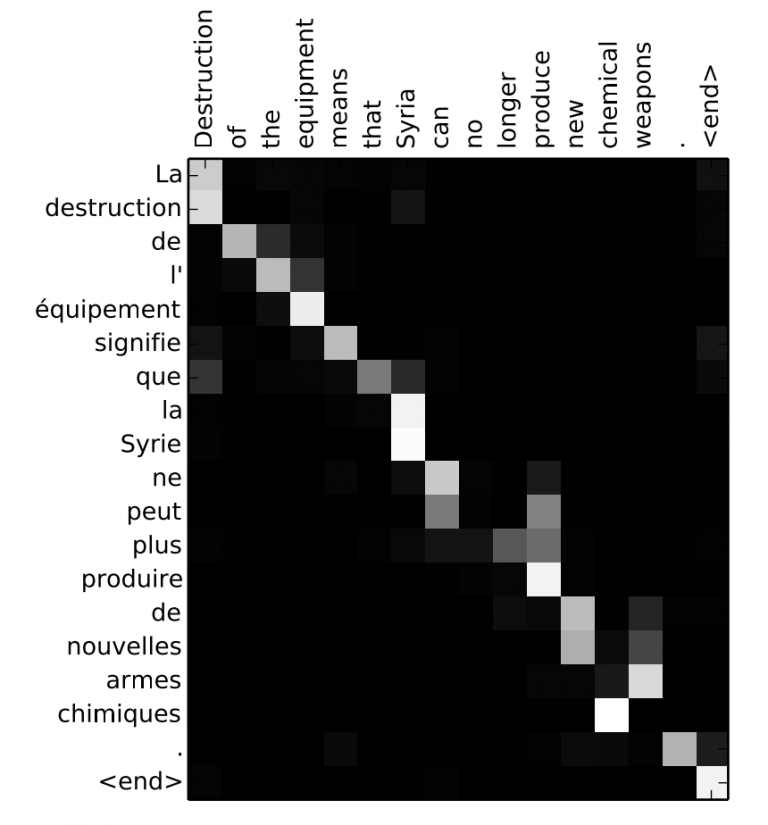
\includegraphics[scale=0.2]{att_w.png}
  \end{center}
\end{frame}

\section{Edge latents guided graph attention networks}

\begin{frame}
  \frametitle{Graph node classification with attention mechanism}
  \begin{block}{Useful information to classify a node}
    \begin{itemize}
    \item features of the node
    \item features of its neighbor nodes
    \item label or prediction of its neighbor nodes
    \end{itemize}
  \end{block}
  \begin{block}{Graph attention network}
    \begin{itemize}
    \item aggregate node features using multiple attention layers
    \item simutaneously classify all nodes of a graph
    \item neighbor label or prediction are aggregated through back-propagation
    \end{itemize}
  \end{block}
\end{frame}

\begin{frame}
  \frametitle{Graph attention network}
  \begin{center}
    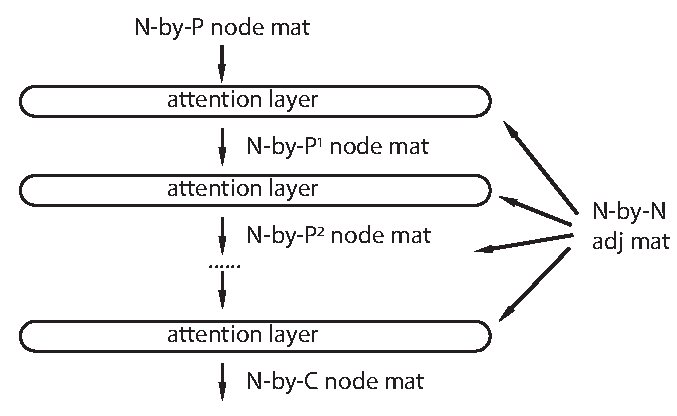
\includegraphics[scale=0.8]{gat_overview.pdf}
  \end{center}
\end{frame}

\begin{frame}
  \frametitle{Graph attention mechanism}
  \begin{center}
    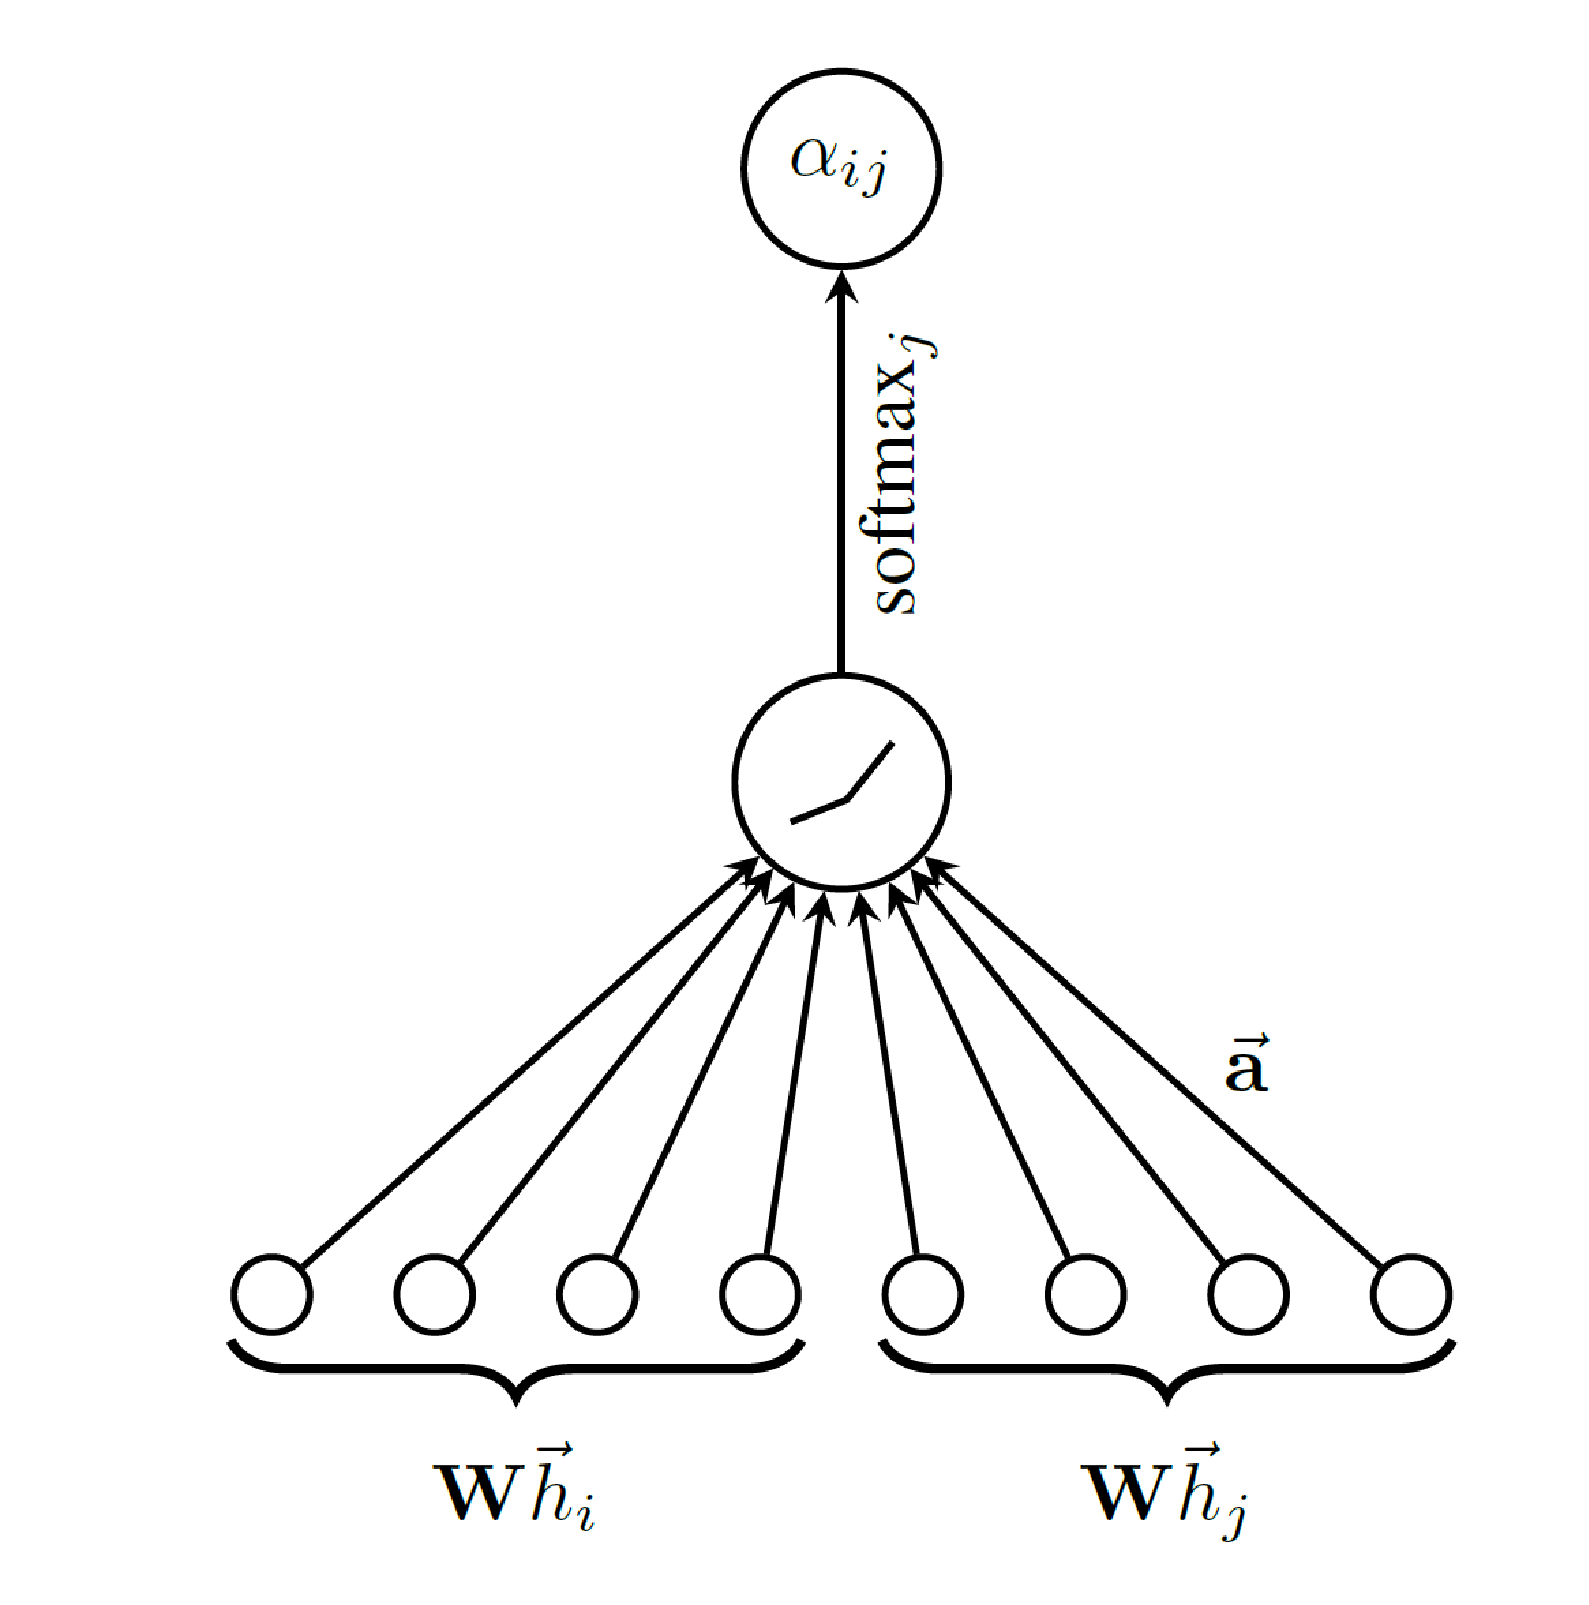
\includegraphics[scale=0.15]{attend.pdf}
    \begin{displaymath}
      \alpha_{ij}=\frac{\exp\left(\mathrm{LeakyReLU}\left(\vectorsym{a}^T\left[\matrixsym{W}\vectorsym{h}_i\parallel{}\matrixsym{W}\vectorsym{h}_j\right]\right)\right)}{\sum_{j\in\mathcal{N}_i}\exp\left(\mathrm{LeakyReLU}\left(\vectorsym{a}^T\left[\matrixsym{W}\vectorsym{h}_i\parallel{}\matrixsym{W}\vectorsym{h}_j\right]\right)\right)}
    \end{displaymath}
  \end{center}
\end{frame}

\begin{frame}
  \frametitle{Multi-head attention}
  \begin{center}
    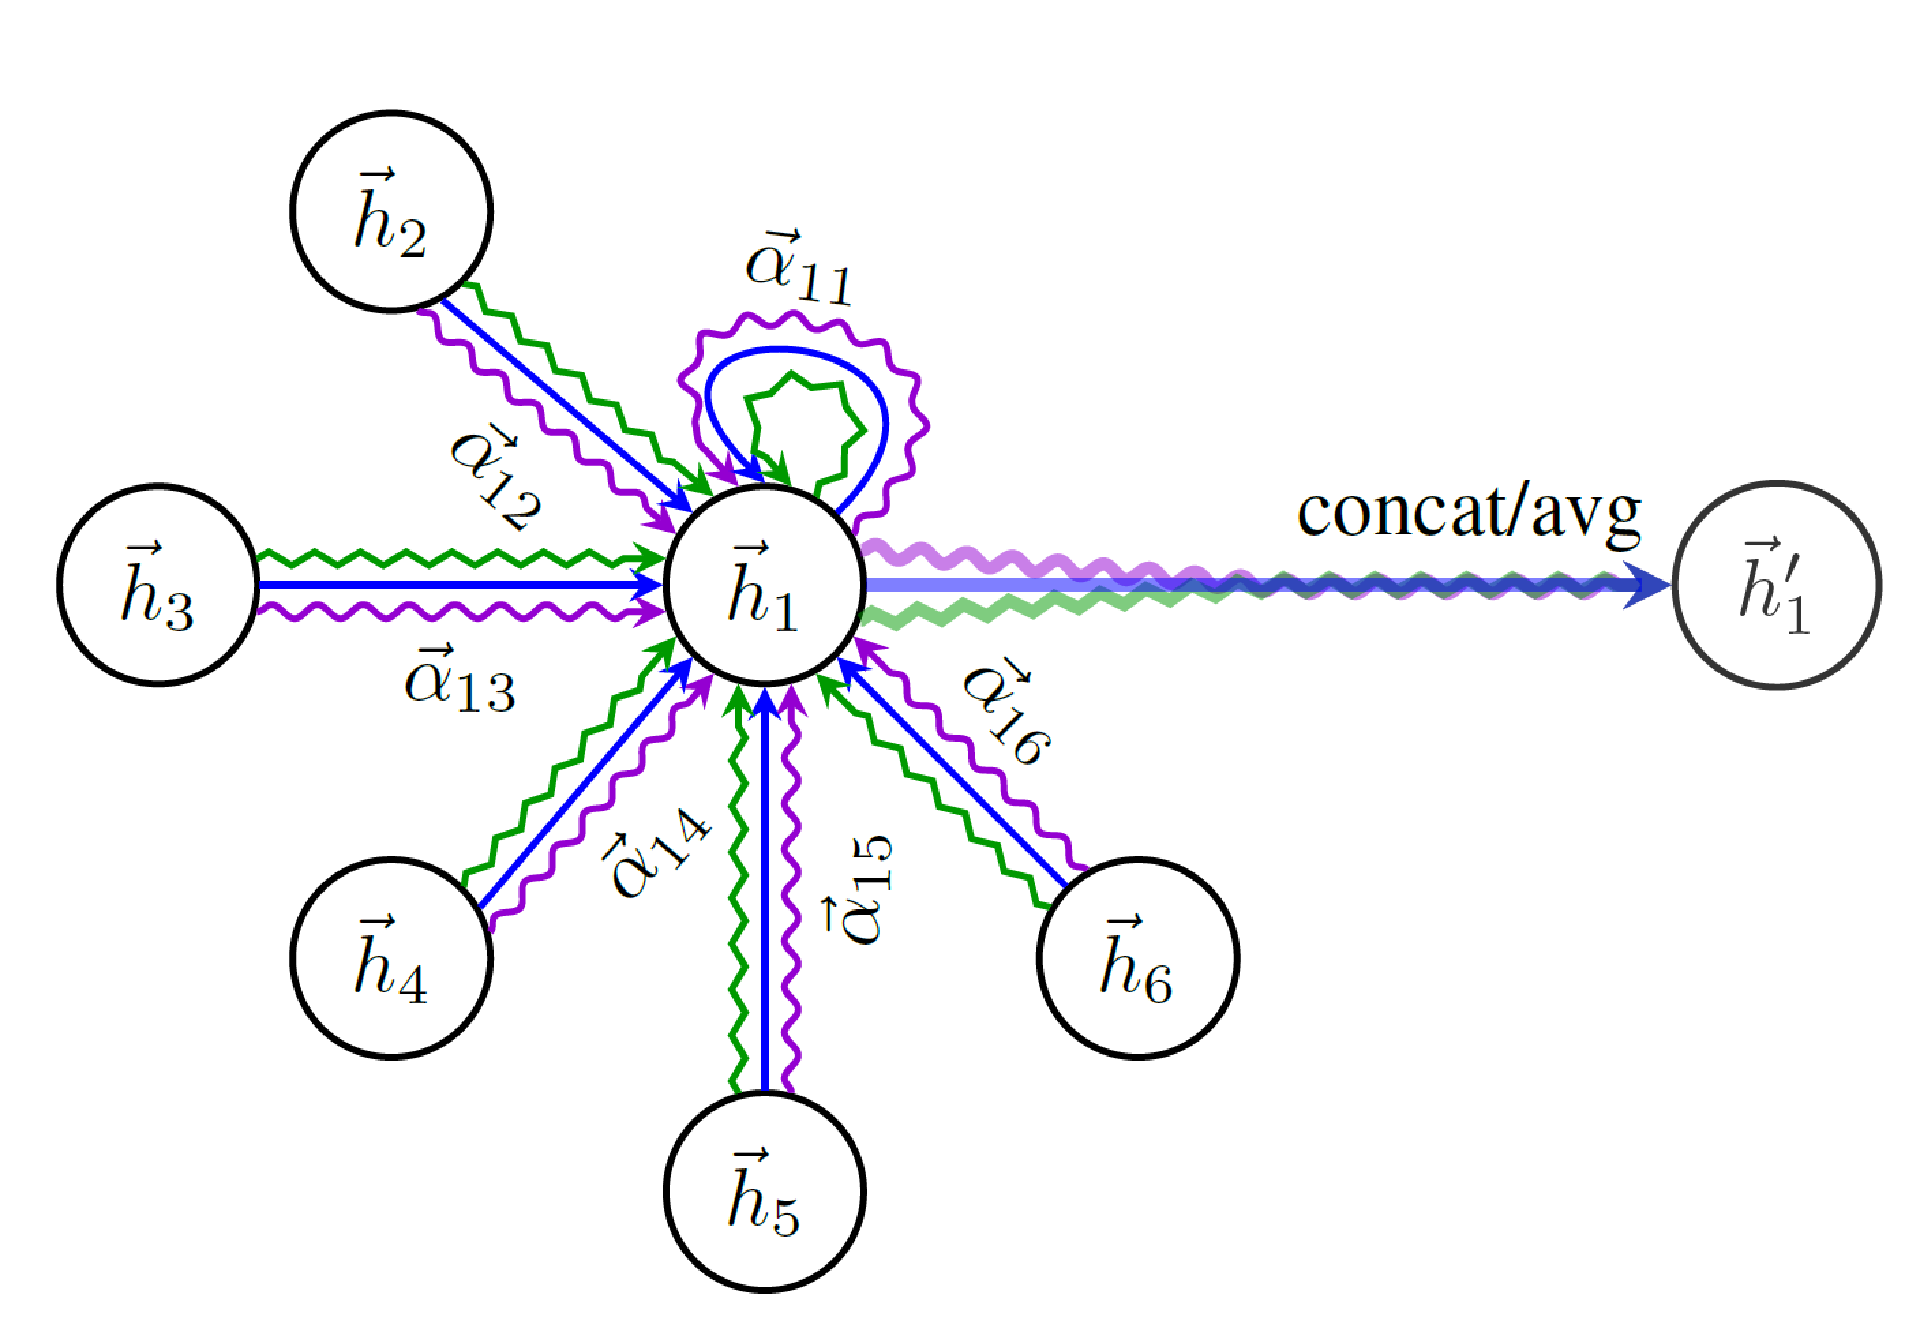
\includegraphics[scale=0.3]{multi_head.pdf}
  \end{center}
\end{frame}

\begin{frame}
  \frametitle{Edge guided graph attention network}
  \begin{center}
    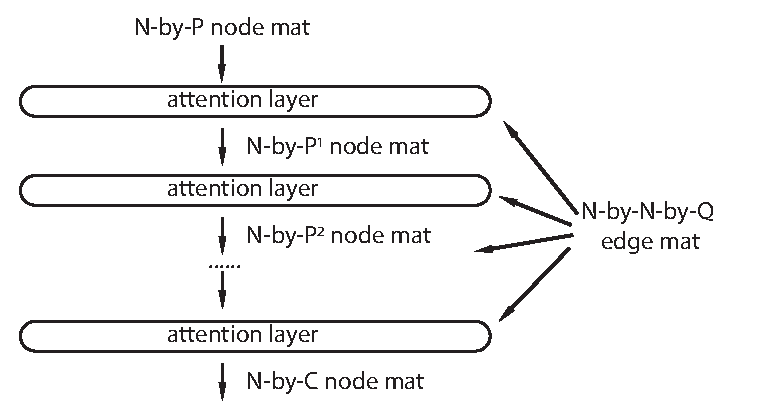
\includegraphics[scale=0.8]{egat_overview.pdf}
  \end{center}
\end{frame}

\begin{frame}
  \frametitle{Edge latents guided attention}
  \begin{itemize}
  \item For different type of edges, attention functions are different
  \item Edge types are represented by edge latent variables
  \end{itemize}
  \begin{center}
    \begin{displaymath}
      \alpha_{ij}=\frac{\exp\left(\mathrm{LeakyReLU}\left(\sum_l\left(\vectorsym{a}_l^T\left[\matrixsym{W}\vectorsym{h}_i\parallel{}\matrixsym{W}\vectorsym{h}_j\right]+\vectorsym{v}_l\vectorsym{g}_{ij}\right)\right)\right)}{\sum_{j\in\mathcal{N}_i}\exp\left(\mathrm{LeakyReLU}\left(\sum_l\left(\vectorsym{a}_l^T\left[\matrixsym{W}\vectorsym{h}_i\parallel{}\matrixsym{W}\vectorsym{h}_j\right]+\vectorsym{v}_l\vectorsym{g}_{ij}\right)\right)\right)}
    \end{displaymath}
  \end{center}
\end{frame}

\section{Results}

\begin{frame}
  \frametitle{Cora dataset}
  \begin{table}
    \centering
    \begin{tabular}{|c|c|}
      \hline
      \# Nodes & 2708\\
      \# Edges & 5429\\
      \# Features/Node & 1433\\
      \# Features/Edge & 2\\
      \# Classes & 7\\
      \# Training Nodes & 140\\
      \# Validation Nodes & 500\\
      \# Test Nodes & 1000\\
      \hline
    \end{tabular}
    \caption{Summary of cora dataset}
    \label{tab:cora}
  \end{table}
\end{frame}

\begin{frame}
  \frametitle{Experimental Results}
  \begin{table}
    \centering
    \begin{tabular}{|c|c|}
      \hline
      Method & Accuracy\\
      MLP & $55.1\%$\\
      ManiReg \cite{belkin_manifold_2006} & $59.5\%$\\
      SemiEmb \cite{weston_deep_2012} & $59.0\%$\\
      LP \cite{zhu_semi-supervised_2003} & $68.0\%$\\
      DeepWalk \cite{perozzi_deepwalk:_2014}& $67.2\%$\\
      ICA \cite{getoor_link-based_2005}& $75.1\%$\\
      Planetoid \cite{yang_revisiting_2016}& $75.7\%$\\
      Chebyshev \cite{defferrard_convolutional_2016}& $81.2\%$\\
      GCN \cite{kipf_semi-supervised_2016}& $81.5\%$\\
      MoNet \cite{monti_geometric_2017}& $81.7\pm{}0.5\%$\\
      GAT & $83.0\pm{}0.7\%$\\
      EGAT & $83.4\pm{}0.6\%$\\
      \hline
    \end{tabular}
    \caption{Summary of results}
    \label{tab:result}
  \end{table}
\end{frame}
\section{Future dirctions}

\begin{frame}
  \frametitle{Future directions}
  \begin{itemize}
  \item Apply to problems with more edge information
  \item Address problems with large graphs
  \item Combine with GCN
  \item Apply to image semantic segmentation (FCN/MS-D + EGAT)
  \end{itemize}
\end{frame}

\begin{frame}
  \frametitle{Semantic segmentation}
  \begin{center}
    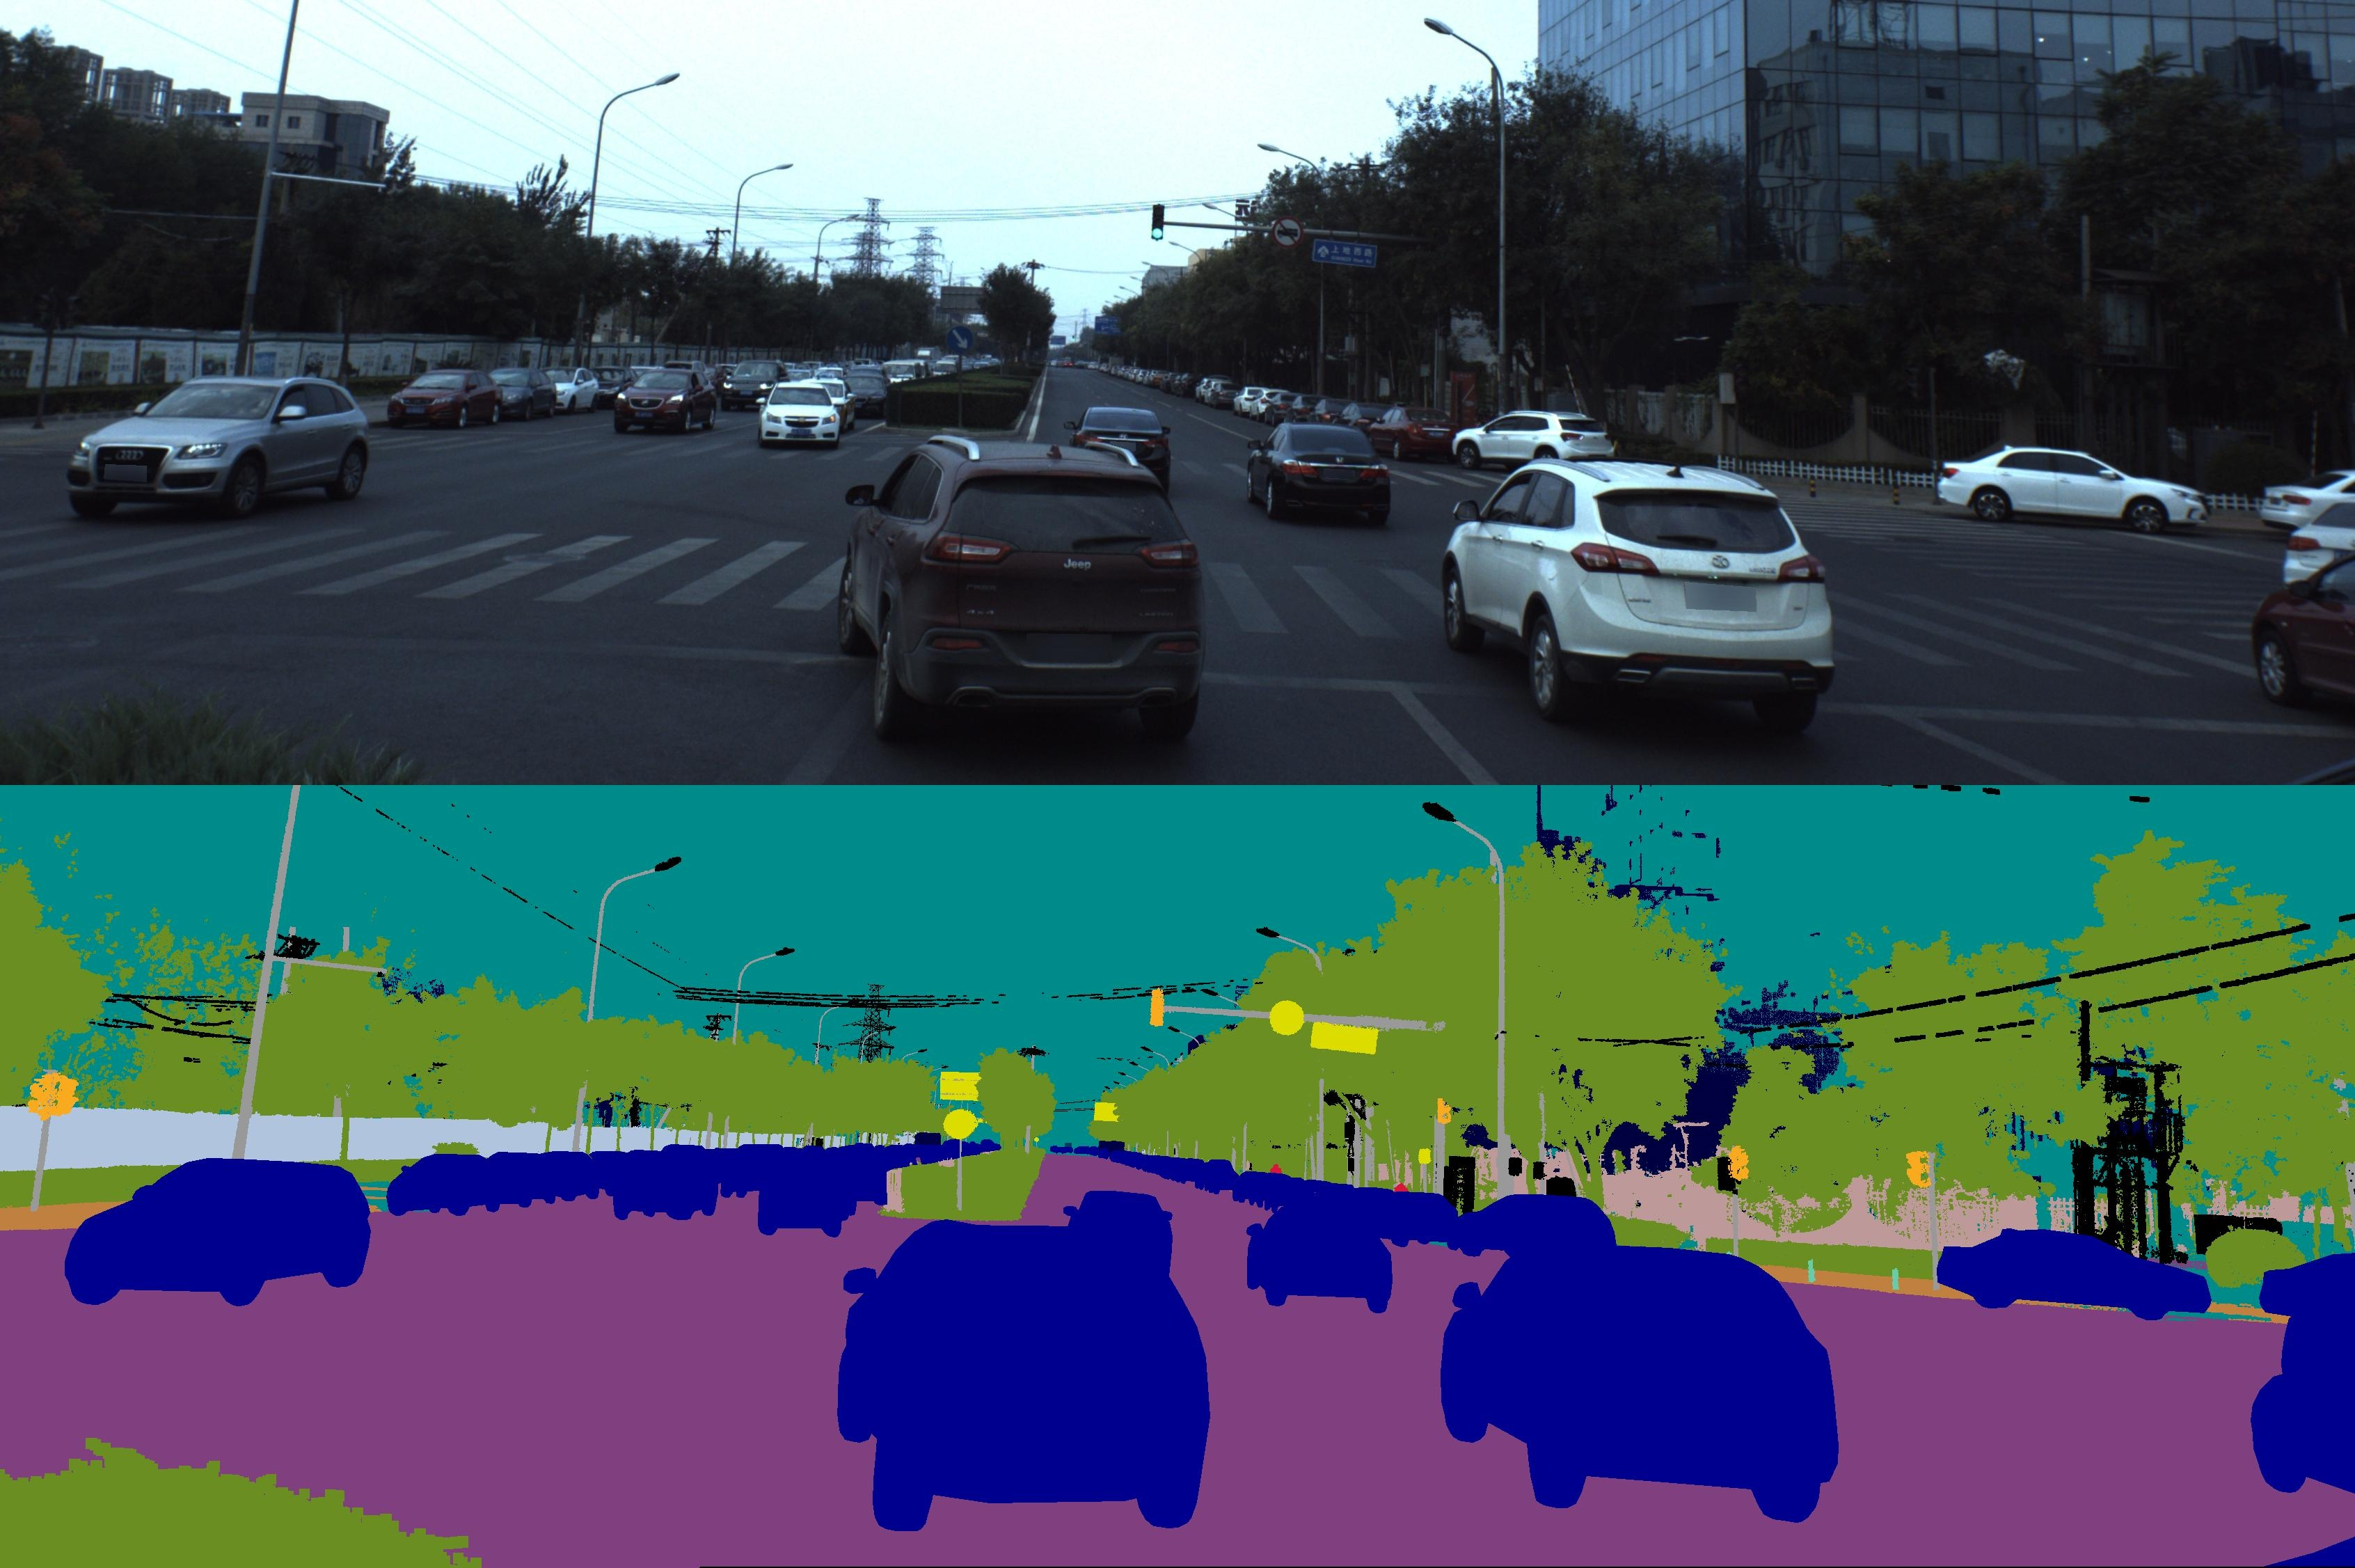
\includegraphics[scale=0.08]{semantic_segmentation.jpg}
  \end{center}
\end{frame}

\begin{frame}
  \frametitle{Semantic segmentation as node classification}
  \begin{block}{Current state-of-the-art method}
    \begin{itemize}
    \item Convolution based
    \item Fully CNN or MS-D (Mixed scale dense CNN)
    \item Convolution weights are shared by all pixel position
    \end{itemize}
  \end{block}
  \begin{block}{Promising EGAT based method}
    \begin{itemize}
    \item Model the problem as a graph node classification
    \item Fully CNN or MS-D for feature learning
    \item EGAT for feature aggregation and pixel classification
    \end{itemize}
  \end{block}
\end{frame}

\begin{frame}[allowframebreaks]
  \frametitle{References}
  \bibliographystyle{ieeetr}
  \tiny
  \bibliography{ref}
\end{frame}

\end{document}

%%% Local Variables:
%%% mode: latex
%%% TeX-master: t
%%% End:
